\documentclass[a4paper,12pt]{jarticle}
\usepackage[dvipdfmx]{graphicx}
\usepackage{url}

\title{CL演習ガイド \#12 レポート\\HTML/CSSによるWebページ作成}
\author{石田 幸太}
\date{2025年7月11日}

\begin{document}

\maketitle

\section{はじめに}
本レポートでは、CL演習ガイド\#12で学習したHTML/CSSによるWebページ作成について報告する。
演習では、HTML文書の基本構造、CSSによるスタイル設定、Webページの公開手順について実践的に学習した。

\section{演習1: HTML基本タグの学習}
演習1では、HTML文書の基本構造を学習した。以下の要素について理解を深めた。

\begin{itemize}
\item HTML文書の基本構造(DOCTYPE、html、head、body)
\item 見出し要素(h1、h2等)の使い方
\item 段落要素(p)とテキストの配置
\item 整形済みテキスト(pre)の表示方法
\end{itemize}

各HTML要素は、文書の構造を明確にし、意味的なマークアップを可能にする。
見出し要素は情報の階層を表現し、段落要素は文章の論理的な区切りを示す。

\section{演習2: CSS基本スタイルの学習}
演習2では、CSSによるスタイル設定について学習した。以下のプロパティを実装した。

\begin{itemize}
\item \texttt{color}: 文字色の指定(blue)
\item \texttt{text-decoration}: 文字装飾の指定(underline)
\item \texttt{text-indent}: 段落の字下げ設定(5mm)
\item \texttt{background}: 背景色の指定(rgb(180,200,255))
\item \texttt{border}: 枠線の指定(double green 4px)
\end{itemize}

CSSを使用することで、HTMLの構造とは独立してデザインを制御できる。
これにより、文書の見た目を柔軟に調整し、視覚的な表現力を向上させることができる。

\section{演習3: Webページの作成と公開}
演習3では、実際のWebページファイルを作成し、ブラウザでの表示を確認した。
以下のコードを実行した。
\begin{verbatim}
<!DOCTYPE html>
<html lang="ja">
<head>
\end{verbatim}

\begin{figure}[htbp]
\begin{center}
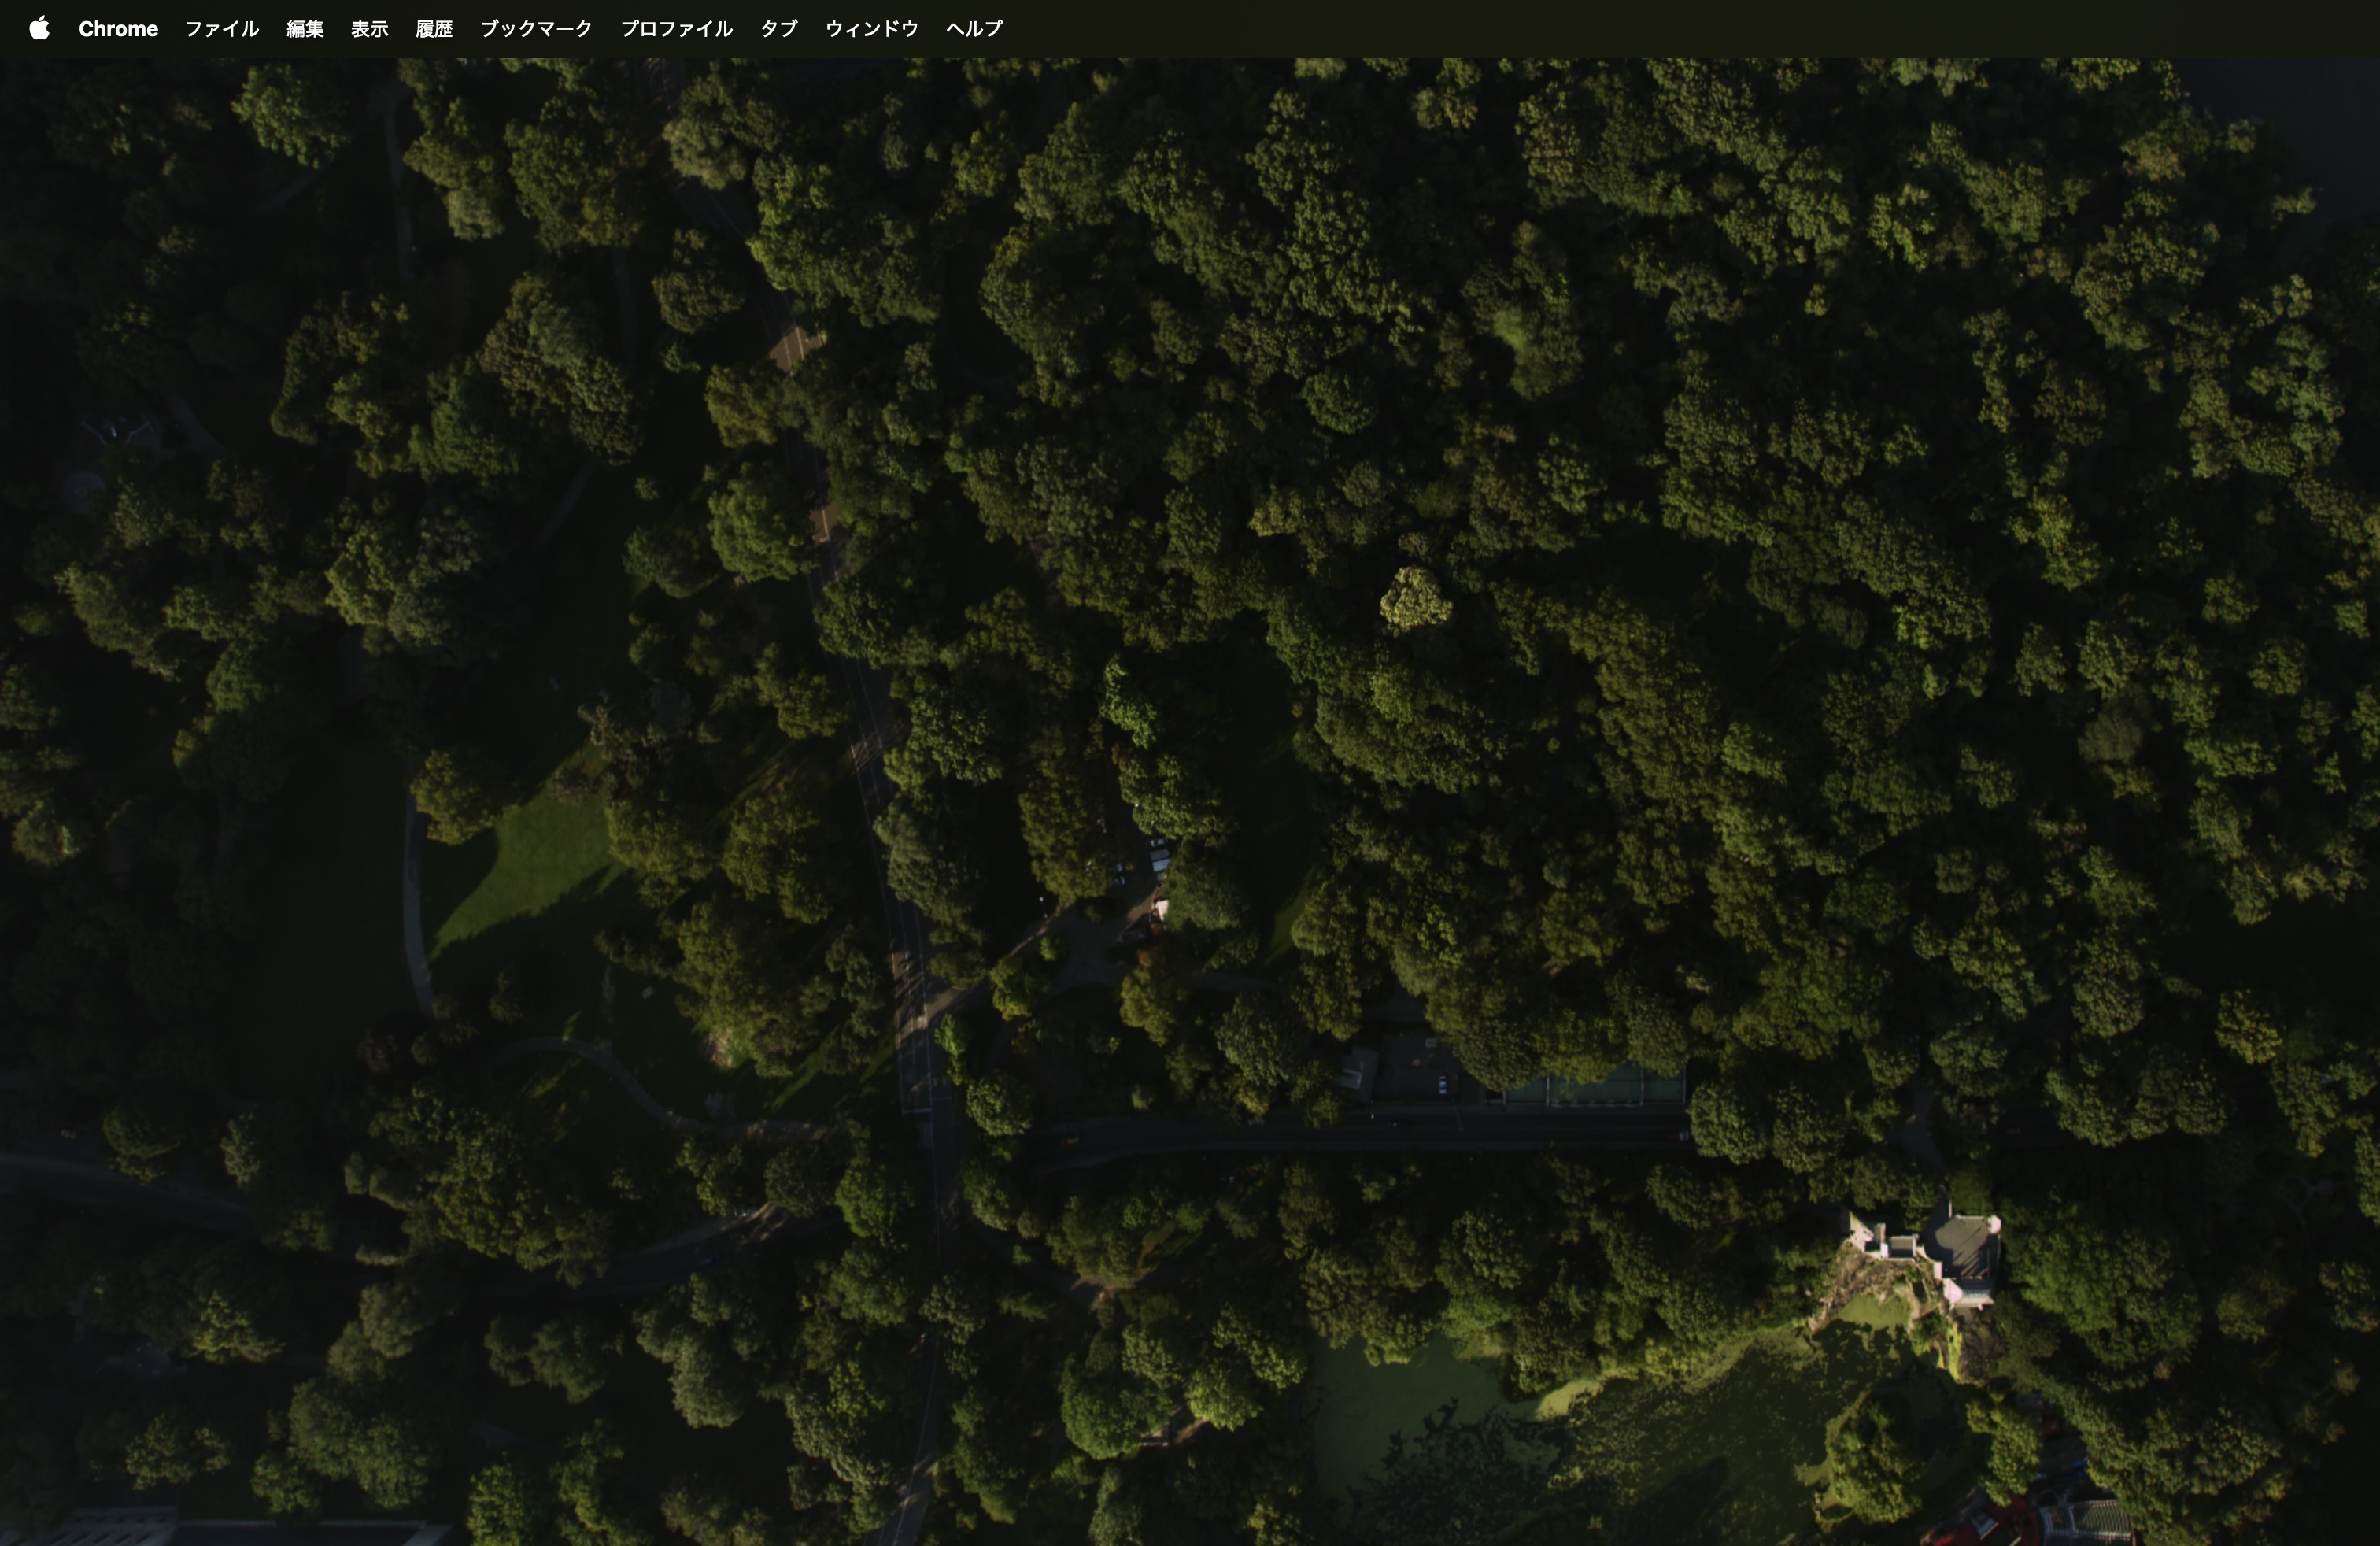
\includegraphics[width=12cm]{webpage_screenshot.png}
\caption{作成したWebページの表示画面}\label{fig1}
\end{center}
\end{figure}

図\ref{fig1}に示すように、作成したWebページでは以下の要素が正しく表示されていることを確認できた。
\begin{itemize}
\item 青色でアンダーライン付きの見出し
\item 水色の背景色と字下げが設定された段落
\item 緑色の二重線枠で囲まれた整形済みテキスト
\item 箇条書きリストの表示
\end{itemize}

\section{考察}
HTMLのheadタグ内は設定をするためのスペース、body内は実際に画面に表示するためのスペースであることだと整理した。
また、Google、firefoxなどの検索エンジン、アクセシビリティツールに対しても理解しやすい文書を作成することができることを学んだ。

CSSによるスタイル設定では、文書の視覚的な表現を柔軟に制御できることを学んだ。
特に、色彩やレイアウトの調整により、情報の階層や重要度を視覚的に示すことができることを学んだ。
また、今後の学習では、より複雑で動きのあるスタイリング技術やレスポンシブデザインについても学習していきたいと思った。

\section{まとめ}
CL演習ガイド\#12を通じて、HTML/CSSによるWebページ作成の基礎を習得した。
HTML文書の構造化とCSSによるスタイル設定の重要性を理解し、
実際のWebページ制作に必要な基本的なスキルを身につけることができた。

\end{document} 